\documentclass[11pt,a4paper,oneside,table,xcdraw]{article}

% CREATED BY DAVID FRISK, 2015


% BASIC SETTINGS

\usepackage{url}
\usepackage{lastpage}								% Get the number of pages
\usepackage{moreverb}								% List settings
\usepackage{textcomp}								% Fonts, symbols etc.
\usepackage{lmodern}								% Latin modern font
\usepackage{helvet}									% Enables font switching
\usepackage[T1]{fontenc}							% Output settings
\usepackage[english]{babel}							% Language settings
\usepackage[utf8]{inputenc}							% Input settings
\usepackage[table]{xcolor} 							% Table colors
\definecolor{light-gray}{gray}{0.96}			% Defining a very light gray for a table

\usepackage{amsmath}								% Mathematical expressions (American mathematical society)
\usepackage{amssymb}								% Mathematical symbols (American mathematical society)
\usepackage{graphicx}								% Figures
\usepackage{subfig}									% Enables subfigures

\usepackage{listings}								% Enables source code listings
\usepackage{xparse}								% Enables in-line code
\NewDocumentCommand{\codeword}{v}{ % Enables in-line code
	\texttt{\textcolor{blue}{#1}}
}
\usepackage{chemfig}								% Chemical structures
\usepackage[top=3cm, bottom=3cm,
			inner=3cm, outer=3cm]{geometry}			% Page margin lengths			
\usepackage{eso-pic}								% Create cover page background
\newcommand{\backgroundpic}[3]{
	\put(#1,#2){
	\parbox[b][\paperheight]{\paperwidth}{
	\centering
	\includegraphics[width=\paperwidth,height=\paperheight,keepaspectratio]{#3}}}}
\usepackage{float} 									% Enables object position enforcement using [H]
\usepackage{parskip}								% Enables vertical spaces correctly 
\usepackage{minted}
%Code highlighting and formatting
\usepackage{dirtree}
\usepackage{epigraph}
%Appendix
\usepackage[toc,page]{appendix}
\usepackage{wrapfig}
\usepackage{caption}
% OPTIONAL SETTINGS (DELETE OR COMMENT TO SUPRESS)

% Disable automatic indentation (equal to using \noindent)
\setlength{\parindent}{0cm}                         


% Caption settings (aligned left with bold name)
% \usepackage[labelfont=bf, textfont=normal,
%			justification=justified,
%			singlelinecheck=false]{caption} 		

		  	
% Activate clickable links in table of contents  	
\usepackage{hyperref}								
\hypersetup{colorlinks, citecolor=black,
   		 	filecolor=black, linkcolor=black,
    		urlcolor=black}


% Define the number of section levels to be included in the t.o.c. and numbered	(3 is default)	
\setcounter{tocdepth}{5}							
\setcounter{secnumdepth}{5}	


% Chapter title settings
\usepackage{titlesec}		
\titleformat{\chapter}
  {\Large\bfseries}{{\fontsize{35pt}{1em} {\thechapter}}}{1ex}{}[]


% Header and footer settings (Select TWOSIDE or ONESIDE layout below)
\usepackage{fancyhdr}
\pagestyle{fancy}
\fancypagestyle{plain}{}
\lhead{}
\rhead{}
\renewcommand{\chaptermark}[1]{\markboth{\thechapter.\space#1}{}}


\fancyhf{}
\fancyhead[L]{Rasmus Isager Kruuse\\Human senses and perception miniproject}
\fancyhead[R]{15/01 - 2018\\MED3}
\fancyhead[C]{}
\fancyfoot[C]{\thepage}

\usepackage[final]{pdfpages}
\usepackage{verbatim}
\usepackage{lipsum}
\usepackage{multicol}
% Enable To-do notes
\usepackage[textsize=tiny]{todonotes}   % Include the option "disable" to hide all notes
\setlength{\marginparwidth}{2.5cm} 

\usepackage{tikz}
\usetikzlibrary{mindmap,trees}
\usepackage{nameref}

% Supress warning from Texmaker about headheight
\setlength{\headheight}{30pt}		

\newcommand{\HRule}{\rule{\linewidth}{0.5mm}}

\usepackage[normalem]{ulem}
\useunder{\uline}{\ul}{}

\usepackage{tocbibind}

\usepackage{tikz}
\usepackage{pgf-pie}
\usepackage{pgfplots}
\pgfplotsset{width=12cm,compat=1.11}
\pgfplotsset{
	cycle list={red\\blue\\},
}
\usepgfplotslibrary{statistics}




\usepackage[natbibapa]{apacite} 

\begin{document}

\begin{titlepage}
\newgeometry{top=3cm, bottom=3cm,
			left=2.25 cm, right=2.25cm}	% Temporarily change margins		
			
% Cover page background 
\AddToShipoutPicture*{\backgroundpic{-4}{56.7}{figure/Frontpage/frontpage-aau.pdf}}
\addtolength{\voffset}{2cm}

% Cover picture 		
\begin{figure}[H]
\centering
\vspace{2cm}	% Adjust vertical spacing here

\includegraphics[width=0.99\linewidth]{figure/Frontpage/gardenposterCropped.png}
\end{figure}

% Cover text
\mbox{}
\vfill
\renewcommand{\familydefault}{\sfdefault} \normalfont % Set cover page font
\HRule\\[0.1cm]
\textbf{{\small Human Senses and Perception\\ {\Huge Vection}}} \hspace{0.15cm}\hspace{0,15cm}{\huge \color{gray}and other types of illusory motion}\\
\HRule\smallskip{}

\Large by \LARGE Rasmus Isager Kruuse\\
\Large stdnr: 20163929\\\\


\today
\renewcommand{\familydefault}{\rmdefault} \normalfont % Reset standard font
\end{titlepage}




\todo{Put in front page}
	\pagenumbering{arabic}

\section{Introduction - what is vection}
You are sitting on a train waiting at the station, zoned out, staring into the middle distance. When your trains set in motion, it takes you a few seconds to realize that it was actually the train across from you that moved. Your brain played tricks on you. This trick is called vection, and everyone has experienced it at some point in thier life. This paper aims to explain why vection happens, by introducing the relevant theory and and goes on to compare vection to other types of illusory self motion. 
\section{What \textit{is} vection?}
One of the problems with the term vection, is that it has been used to describe many different things by different researchers. \cite{challenges} published a paper in which they stated four challenges that vection research currently faces. One of these is the lack of a concrete definition. They gave examples of four different definitions that was used in research. As such one should clearly define which definition that is used. In this paper i use the 1st definition, which is.
\begin{quote}
\textit{Vection is a visual illusion of self-motion in a stationary observer}
	\end{quote}
	Following this definition vection can be described more clearly. Vection as referred to in this report is the sensation of self motion that one can get when a large part of the visual field starts moving. This often happens near large objects that such as on a ferry, on a train, or sometimes in a car. For example, if an observer is in a stationary train and the beside it starts moving. It is not uncommon to feel as if you train has started to move instead. This is vection. We are currently unsure whether vection serves a purpose in making controlling self-motion of just arises from the processing of visual data. That is, whether it has some use or is a glitch in the visual system that only occurs under very particular conditions that never happened before modernity\todo{citation maybe}. 
	\section{Theory}
To understand why certain conditions can trick the human perception system into feeling self motion where there is none, we must first understand how the humans perceive motion, and why this causes no problems under normal conditions. This section covers the theory of human motion perception. \\
\todo{Answer the following questions 3. Vection. Explain what vection is and how it differs from other types of illusory self motions one might experience. When and how can we experience vection? What determines whether it happens or not and how long the sensation lasts? }	
\subsection{Vision based motion detection}

Since a three dimensional world is projected onto a two dimensional surfaces(the retina), motion can be though of as an image moving around the retina. If a point is somewhere at one point in time, and elsewhere at another, it must have moved. Thinking of this in terms of receptive fields, if one receptive field gives a powerful response, and a few milliseconds later a nearby receptive field also gives a powerful response. Then perhaps whatever caused that response has moved, as illustrated in Figure \ref{fig:overtime}.
\begin{figure}[H]
		\centering
		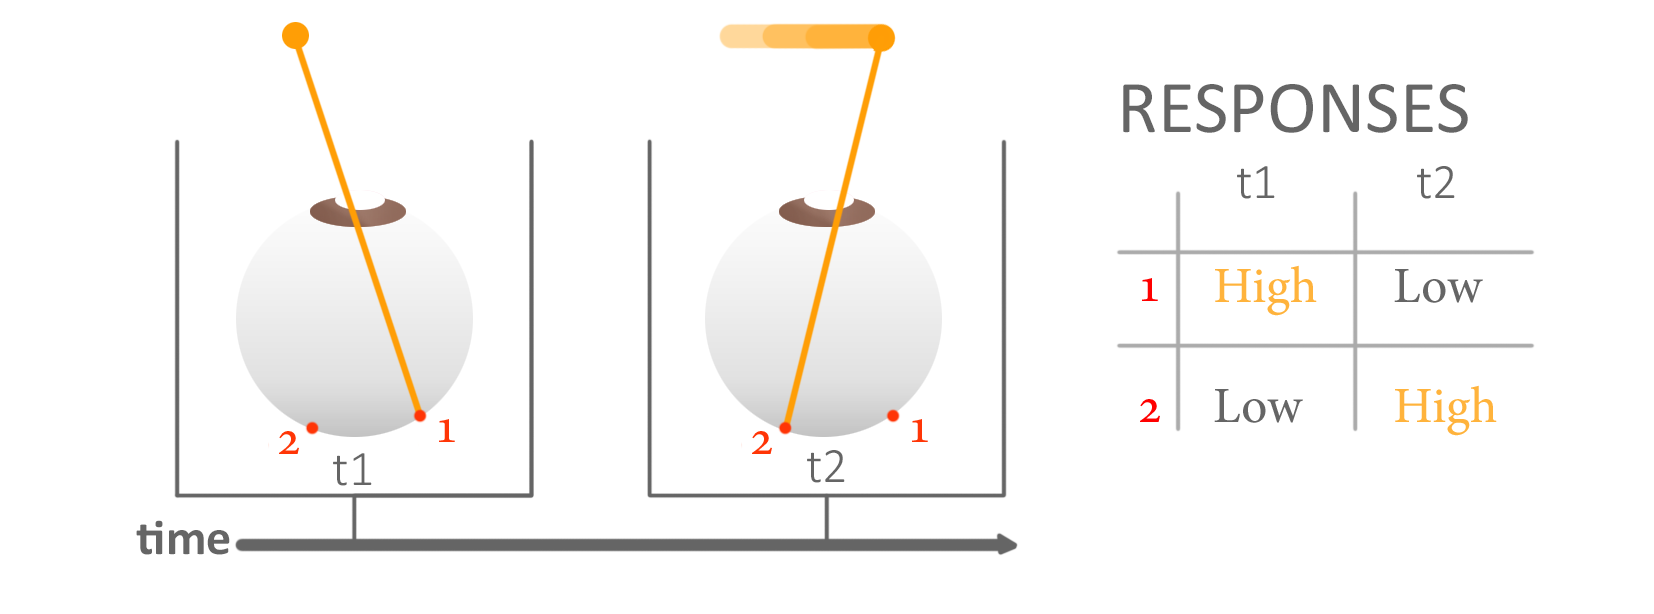
\includegraphics[width=1\linewidth]{figure/overtime.png}
		\caption{In terms of the eye, movement can be understood as points moving on the back of the eye}
		\label{fig:overtime}
\end{figure}
In the retina, the back of the eyeball, sit light sensitive cell that respond to light. The output from a number of these can be combined to detect local changes in light, and respond strongly to edges \cite[p. 53]{coursebook}. The section of vision that these cell are responsible for is called their \textit{receptive fields}. The retina has around 1 million receptive fields covering it's field of view, with many of the field types overlapping\cite[p. 64-65]{coursebook}. \cite{Barlow1965} found cells in the retina of rabbits, that gave a powerful responses when an object moved through a specific part of the rabbits vision in one direction, but would give little to no response if the object was moved in the opposite direction. These were named direction sensitive cells, or DS cells. \citet{review} points out that multiple models have been suggested that could explains this behavior. They rely on combining the output of multiple receptive fields.\\\\
If we imagine a neuron N that is connected to two receptive fields f1, and f2. This neuron, N, will only fire if it simultaneously receives a signal from both receptive fields. Now imagine that an object moves across each of the receptive fields in succession. The first field(f1) will fire, and then the second(f2) will fire. However, by the time the signal from f2 reaches N, the signal from f1 has already arrived. This problem is illustrated in Figure \todo{create fig.}. Because the signals do not arrive at the same time, N will not fire.\\\\

Werner \cite{beetle} noted that such a system would respond to motion if the signal from f1 took longer time to reach N, compared to the signal from f2. Figure \todo{Another fig}, represent the system from above but with a delay between f1 and N. As before f1 still fires first, but it does not reach N immediately. When f2 fire, f1's signal is still heading towards N, and the signals now reach N at the same time. Neuron N now fire, signaling motion. There are a few things to note. (1) the delay is static. As such, each particular circuit is attuned to a specific speed. (2) f1 and f2 do not move, as such N only detects movement in a certain direction. (3) because the responses of the fields are dependent upon the moving object's brightness, N can not distinguish between a bright object moving at an angle between the fields, and a dim object moving in the direction N is sensitive to. (4) If a large  object cover both f1, and f2, both will fire so long as the object is in front of them, meaning that N will fire event if there no motion in a large object.
\\\\
These problem have led to the suggesting that these type of circuits operate in pairs of two. With two neurons (N1,N2) sensitive to motion in opposite direction as shown in Figure \todo{fig}. In this circuit the final output OUT is a neuron which normally fires at a baseline rate. OUT get an excitatory signal, which causes it to fire more often, from N2, and an inhibitory which causes it to fire less often from N1. In other words, if N2 fires the output will be larger, and if N1 fires the output will be smaller, and if none or both fire the output will be the normal baseline. This change solves some of the problems with the circuit above. (3), in cases where the objects direction is neither in N1 or N2's preferred direction, both will give a weaker signal canceling each other out. (4) In case of a stationary object, both N1 and N2 will again send a similar signal, canceling each other out. This circuit has properties similar to those of the direction sensitive cells in rabbit eyes described by \cite{Barlow1965}.


	\subsection{Direction sensitive neurons}
\iffalse
	As a guideline, someone reading your report should be able to answer the questions/tasks stated for the topic after having read it. The more you understand your topic and can explain it in your own words, the greater the likelihood is that you succeed.\\\\
	Report the theory relevant to your topic and the questions you are to answer. The available course literature (e.g. Yantis \& Abrams, 2017; Wolfe et al., 2015; Snowden, Thompson, \& Troscianko, 2006) are good starting points, but to get more specific information and achieve a higher grade you should also search for and read review articles (e.g. Elliot 2015; Elliott, Vale, Whitaker \& Buckley, 2009), and other relevant information. Use the suggested readings or references listed in your course book as a starting point and search for related articles and articles that have been citing the earlier ones.\\\\
	If you have any questions regarding your report, please contact your teacher in reasonable time before hand in. The weekend of delivery is NOT reasonable.

	\section{Discussion}
	After you have reported the theory and clarified or answered the questions stated in
	the topic you should devote about one page to put this into context. Try to think of
	what it means for everyday life and our usage of digital media. Find examples! What
	should one take into consideration when designing multimedia applications? How can
	you use the knowledge in your semester project?
	Similarly, if you have reported own experiments you also need to put this in
	perspective: Could you have used other approaches, references or theories? Did
	anything go wrong (weaknesses)? What was good (strength)? Create relevant
	subheadings that depict the topics you have extrapolated. 
\fi
\bibliographystyle{apacite}
\bibliography{include/backmatter/bibliography}

\end{document}